\documentclass{article}
\usepackage{graphicx}
\usepackage[]{mdframed}
\usepackage{tabularx}
\usepackage{subfig}
\usepackage{placeins}
\usepackage{float}

\graphicspath{ {./images/} }
\usepackage[a4paper, total={6in, 8in}]{geometry}


\author{Sidharth Babu, SNB2593 \and Tianda Huang, TH32684}
\title{ECE 361E: Homework 3}

\begin{document}
\begin{mdframed}
    \maketitle
\end{mdframed}
\pagebreak

\section*{Problem 1}
\subsection*{Question 2}
\begin{tabularx}{\textwidth} { 
    | >{\centering\arraybackslash}X 
    | >{\centering\arraybackslash}X 
    | >{\centering\arraybackslash}X
    | >{\centering\arraybackslash}X
    | >{\centering\arraybackslash}X
    | >{\centering\arraybackslash}X
    | >{\centering\arraybackslash}X 
    | }
    \hline
    Model & Training Accuracy(\%) & Test Accuracy (\%) & Total time for training (s) & Number of Trainable Params & Floating Point Operations & GPU memory during training (mb)\\
    \hline
    VGG11 & 97.57 & 76.48 & 3011.79 & 9,750,922 & 306,587,648 & 2583 \\
    \hline
    VGG16 & 97.86 & 78.89 & 3622.42 & 14,655,050 & 551,954,432 & 2583 \\
    \hline
    MobileNet & 99.42 & 77.75 & 2211.56 & 3,217,226 & 96,002,048 & 1151\\
    \hline
\end{tabularx}

\subsection*{Question 3}
\begin{figure}[h]
    \centering
    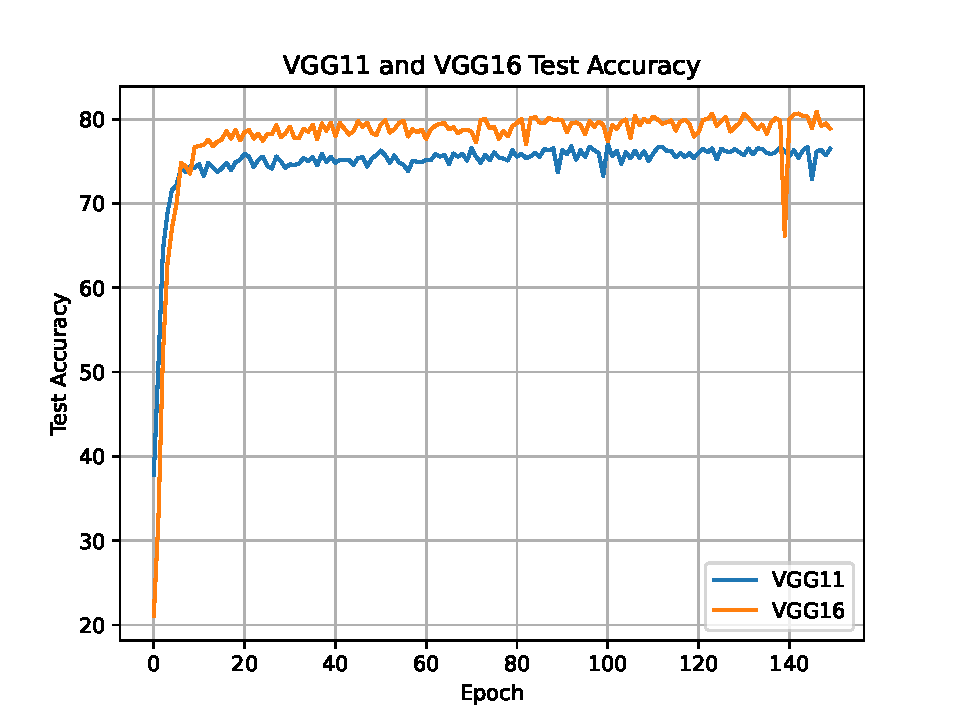
\includegraphics[width=\textwidth]{graphing/vgg11_16_acc.pdf}
    \caption{Test Accuracy of VGG11 and VGG16}
    \label{fig:accuracy}
\end{figure}

VGG16 performs incrementally better than VGG11 on both train and test. However it has 1.5x the amount of trainable parameters and 1.8x the amount of floating point operations. 
The small accuracy boost is not worth the increase in computational complexity, and therefore we would choose VGG11 to train. 

\section*{Problem 2}
\subsection*{Question 2}
\begin{center}
\begin{tabular}{|*{7}{c|}}
    \hline
      & \multicolumn{2}{c|}{Total Inference Time [s]}  & \multicolumn{2}{c|}{RAM memory [MB]} & \multicolumn{2}{c|}{Accuracy[\%]} \\
    \cline{1-7}
      & MC1 & RaspberryPi & MC1 & RaspberryPi & MC1 & RaspberryPi \\
    \hline
    VGG11 & 658.23 & 680.61 & 330 & 171 & 76.48 & 76.48\\
    \hline
    VGG16 & 990.92 & 1172.02 & 352 & 192 & 78.89 & 78.89\\
    \hline
    MobileNet & 491.65 & 329.30 & 302 & 139 & 77.75 & 77.75\\
    \hline
\end{tabular}
\end{center}

\begin{center}
    \begin{tabular}{|*{3}{c|}}
        \hline
        Model & MC1 Total Energy Consumption [J] & RPI total Energy Consumption \\
        \hline
        VGG11 & 6574.78 & 3739.40 \\
        \hline
        VGG16 & 10106.79 & 6381.64 \\
        \hline
        MobileNet & 4196.58 & 1877.45 \\
        \hline
    \end{tabular}
\end{center}
\subsection*{Question 3}
\section*{Problem 3}
\subsection*{BONUS}
The MobileNet model performs the best in terms of composite performance across both platforms.
It is the most energy efficient model, is the fastest model in terms of inference, and has 
accuracy on par with the other two models.
MobileNet's key advantage is the usage of depthwise convolution, which significantly reduces the computation cost of the forward pass on convolutional layers.
Depthwise convolution works by splitting the convolution operation into two steps. First, a single filter is applied to each input channel, which is followed by a pointwise convolution to combine the output channels into one output.
This is significantly faster than convolving one learned filter with the entire input tensor. 

\end{document}